\documentclass{article}
\usepackage{indentfirst}
\usepackage[utf8]{inputenc}
\usepackage[T1]{fontenc}
\usepackage{lmodern}
\usepackage{graphicx}
\usepackage{float}
\usepackage[]{subfigure}
\usepackage{afterpage}

\usepackage[brazilian]{babel}


\usepackage{listings}
\usepackage{color}

\definecolor{dkgreen}{rgb}{0,0.6,0}
\definecolor{gray}{rgb}{0.5,0.5,0.5}
\definecolor{mauve}{rgb}{0.58,0,0.82}

\lstset{frame=tb,
  language=Matlab,
  aboveskip=3mm,
  belowskip=3mm,
  showstringspaces=false,
  basicstyle={\small\ttfamily},
  numbers=none,
  numberstyle=\tiny\color{gray},
  keywordstyle=\color{blue},
  commentstyle=\color{dkgreen},
  stringstyle=\color{mauve},
  breaklines=true,
  breakatwhitespace=true,
  tabsize=4
}


\addtolength{\topmargin}{-.750in}
\addtolength{\textheight}{1.5in}


\title{Simulação 3 - Controle Digital}
\author{Arthur de Matos Beggs - 12/0111098}
\date{}

\begin{document}

%\maketitle

% capa
\begin{titlepage}
    \begin{center}
        \centering
        
\includegraphics[width=.5\linewidth]{images/LogoUnB.jpg}\\[0.1cm]
        {\large \textbf{Universidade De Brasília}}\\[0.2cm]
        {\large \textbf{Departamento De Engenharia Elétrica}}\\[0.2cm]
        {\large \textbf{Controle Digital}}\\[5.1cm]
        {\bf \huge Simulação 3}\\[5.1cm]
    \end{center}
{\large Aluno: \\    Arthur de Matos Beggs ----------------------------------------- 12/0111098 }
\vspace{7mm}
    \begin{center}
        {\large 1º/2020}
    \end{center}
\end{titlepage}

\clearpage % Quebra de página

\setcounter{page}{2}


\section{Questão 1}

    \begin{figure}[H]
       \centering
            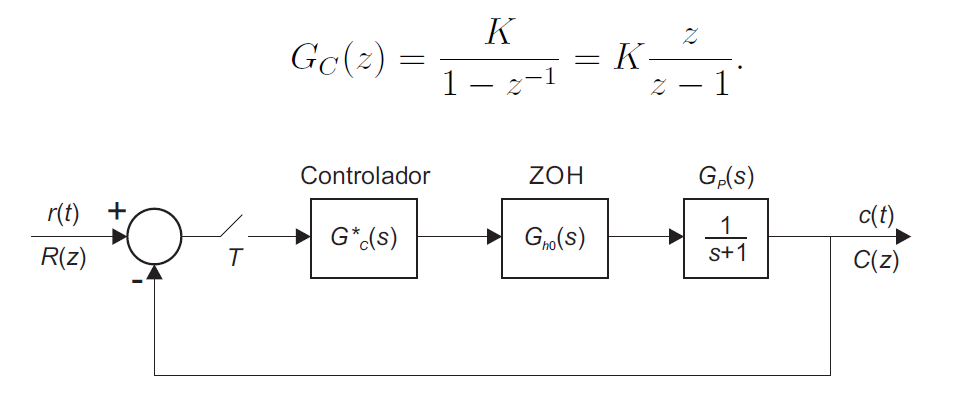
\includegraphics[width=1\linewidth]{images/Diagrama.png}
            \caption{Diagrama e funções de transferência do sistema.}
            \label{fig:diagram}
    \end{figure}

    {\textbf{a)} Para esboçar o LGR para os períodos de amostragem T = 0,5s, T = 1s e T = 2s, o seguinte script foi utilizado:}

\vspace{7mm}
\begin{lstlisting}
s    = tf('s');
Gp   = 1/(s+1);

T1   = 0.5;
z1   = tf('z',T1);
Gc1  = z1/(z1-1);
rl1  = c2d(Gp, T1, 'zoh') * Gc1;

T2   = 1.0;
z2   = tf('z',T2);
Gc2  = z2/(z2-1);
rl2  = c2d(Gp, T2, 'zoh') * Gc2;

T3   = 2.0;
z3   = tf('z',T3);
Gc3  = z3/(z3-1);
rl3  = c2d(Gp, T3, 'zoh') * Gc3;

rlocus(rl1, rl2, rl3);

\end{lstlisting}

    \vspace{7mm}
    {A execução do script gerou o \textit{plot} apresentado na Figura 2.}

    \newpage

    \begin{figure}[H]
       \centering
            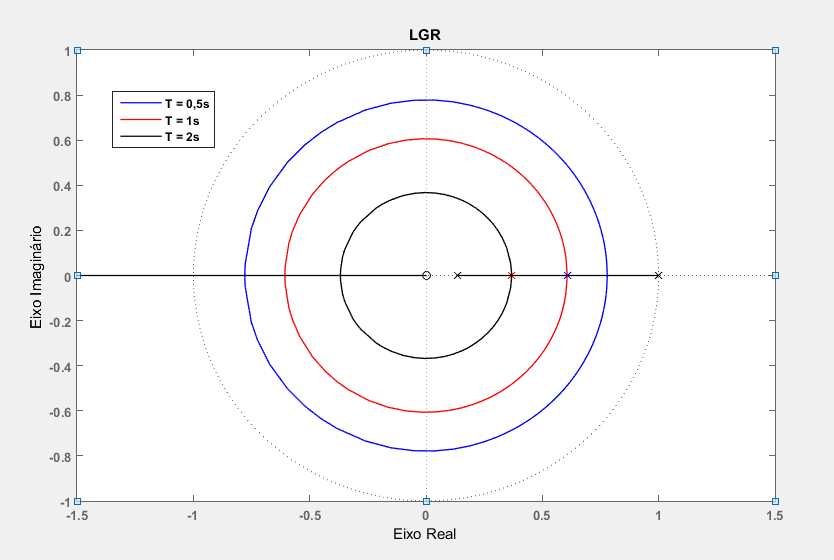
\includegraphics[width=1\linewidth]{images/LGR.png}
            \caption{LGR no plano \textit{z} para T = 0,5s, 1s e 2s.}
            \label{fig:lgr}
    \end{figure}


    \vspace{7mm}
    {\textbf{b)} O valor de K crítico para cada período de amostragem é encontrado graficamente com o auxílio do cursor do Matlab no ponto em que o LGR deixa o círculo de raio unitário. A medida com o cursor apresenta uma imprecisão considerável, e por isso os valores de K crítico obtidos por esse método devem ser interpretados como aproximações.}

    \vspace{7mm}
    \begin{figure}[H]
       \centering
            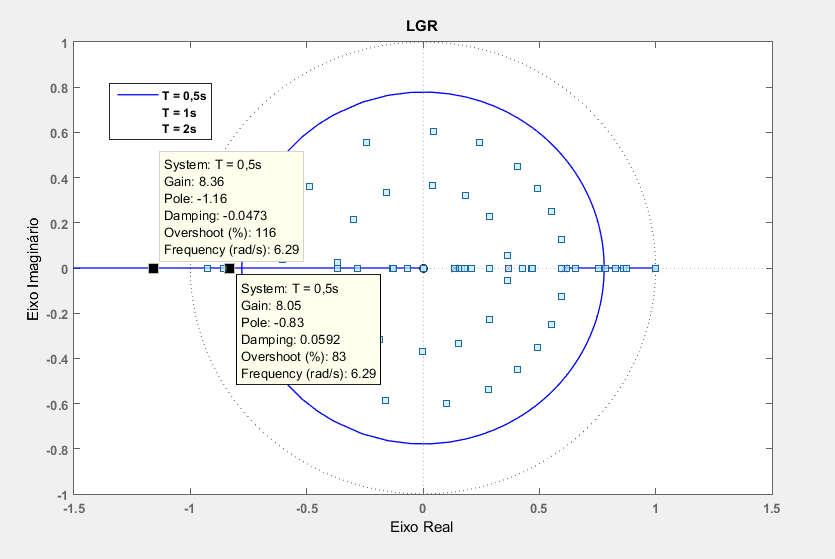
\includegraphics[width=.9\linewidth]{images/LGR_Kcrit05.png}
            \caption{Para T = 0,5s, Kcrit $\approx$ 8,205 (obtido por interpolação).}
            \label{fig:Kcrit05}
    \end{figure}

    \begin{figure}[H]
       \centering
            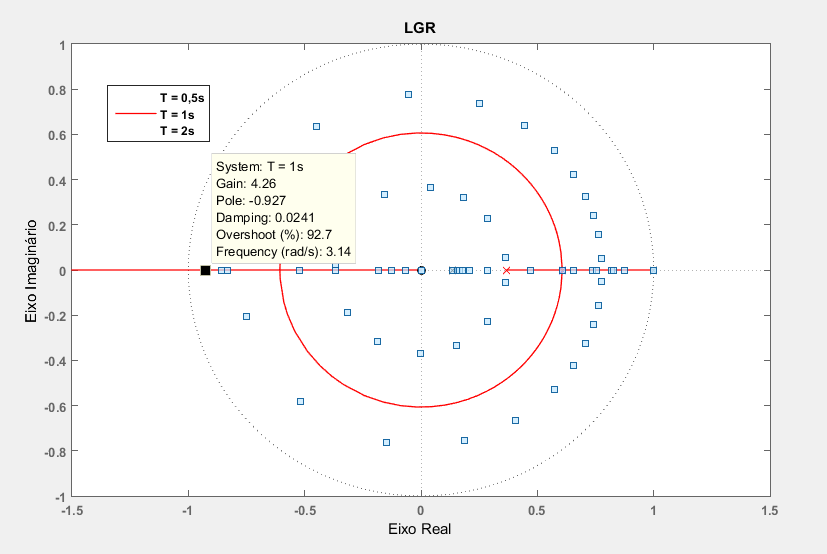
\includegraphics[width=1\linewidth]{images/LGR_Kcrit1.png}
            \caption{Para T = 1s, Kcrit $\approx$ 4,26.}
            \label{fig:Kcrit1}
    \end{figure}

    \begin{figure}[H]
       \centering
            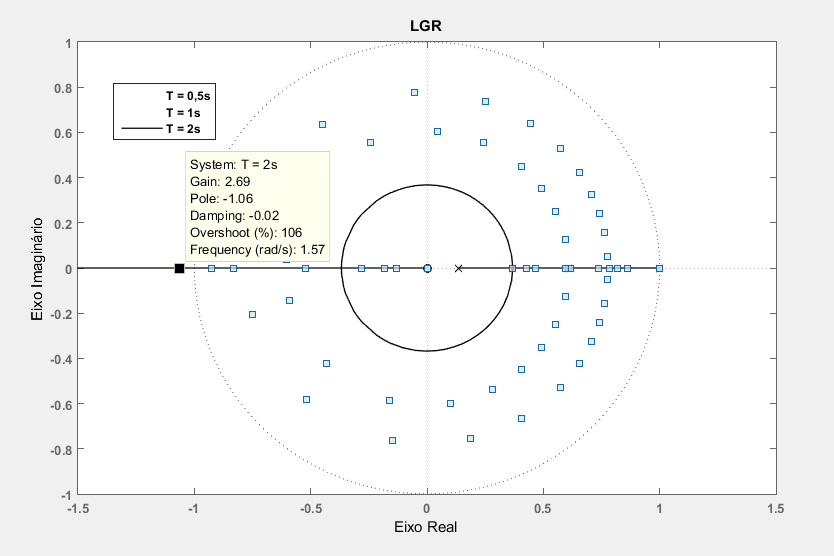
\includegraphics[width=1\linewidth]{images/LGR_Kcrit2.png}
            \caption{Para T = 2s, Kcrit $\approx$ 2,69.}
            \label{fig:Kcrit2}
    \end{figure}

    \clearpage

    {\textbf{c)} Os pólos dominantes de malha fechada no plano \textit{z} quando K = 2 para cada valor de T foram obtidos posicionando o cursor sobre o ganho = 2. A medida com o cursor apresenta uma imprecisão considerável, e por isso os valores dos pólos dominantes obtidos por esse método devem ser interpretados como aproximações.}

    \vspace{7mm}
    \begin{figure}[H]
       \centering
            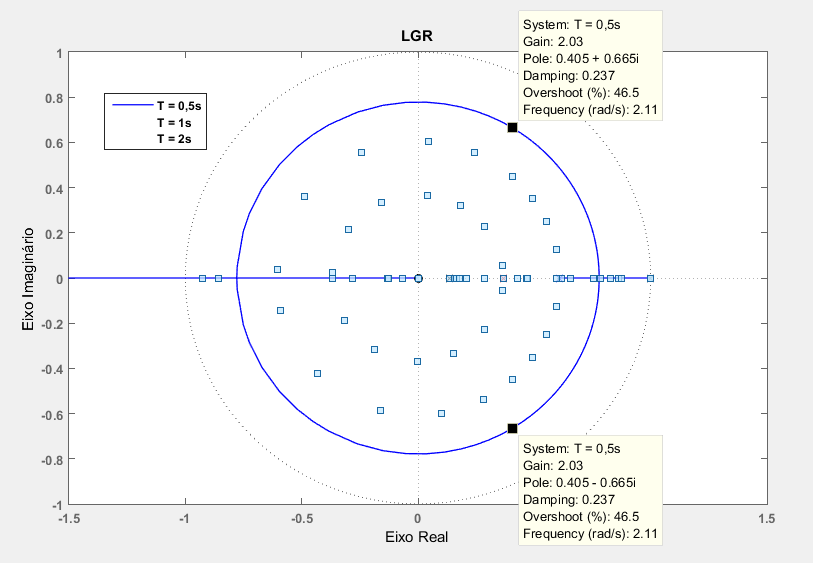
\includegraphics[width=.9\linewidth]{images/LGR_PoloDom05.png}
            \caption{Para T = 0,5s, os pólos dominantes $\approx$ 0,405 $\pm$ 0,665j.}
            \label{fig:poloDom05}
    \end{figure}

    \begin{figure}[H]
       \centering
            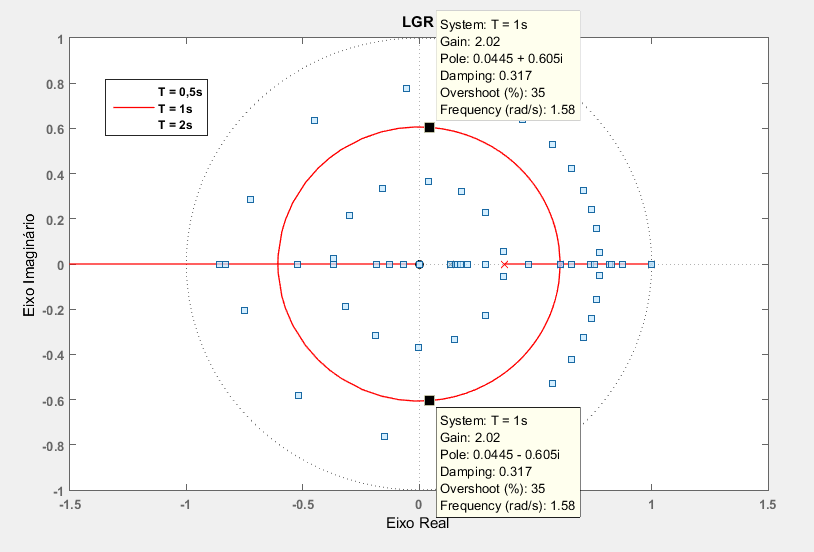
\includegraphics[width=.9\linewidth]{images/LGR_PoloDom1.png}
            \caption{Para T = 1s, os pólos dominantes $\approx$ 0,0445 $\pm$ 0,605j.}
            \label{fig:poloDom1}
    \end{figure}

    \begin{figure}[H]
       \centering
            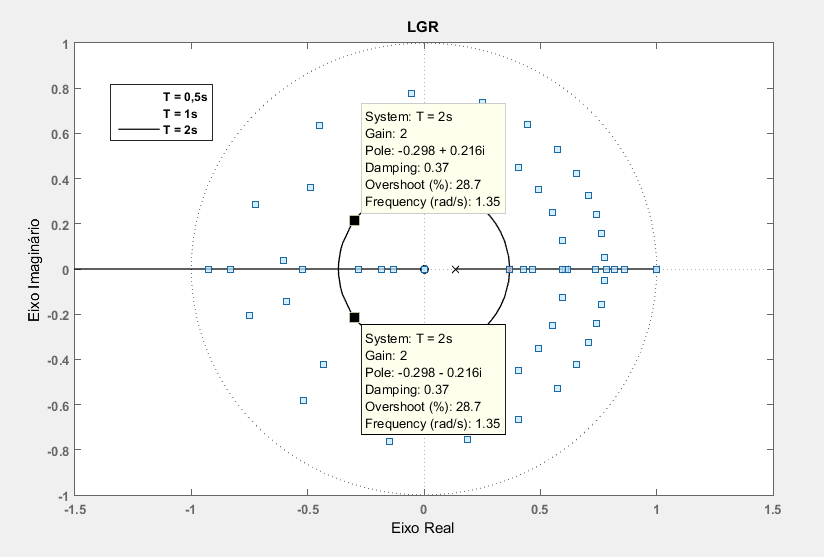
\includegraphics[width=1\linewidth]{images/LGR_PoloDom2.png}
            \caption{Para T = 2s, os pólos dominantes $\approx$ -0,298 $\pm$ 0,216j.}
            \label{fig:poloDom2}
    \end{figure}


    \vspace{7mm}
    {Para as letras \textbf{d} e \textbf{e}, o diagrama do Simulink presente na Fig 9 foi utilizado.}

    \begin{figure}[H]
       \centering
            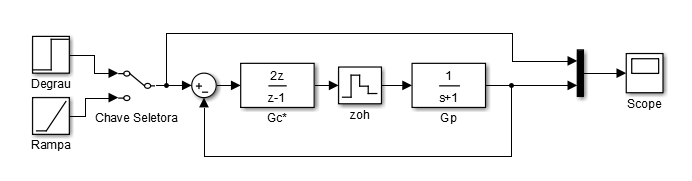
\includegraphics[width=1\linewidth]{images/DiagramaSimulink.png}
            \caption{Diagrama do sistema representado no Simulink.}
            \label{fig:diagSim}
    \end{figure}

    \vspace{14mm}
    {\textbf{d)} As respostas ao degrau do sistema para diferentes tempos de amostragem e K = 2 são apresentadas nas figuras a seguir.}

    \begin{figure}[H]
       \centering
            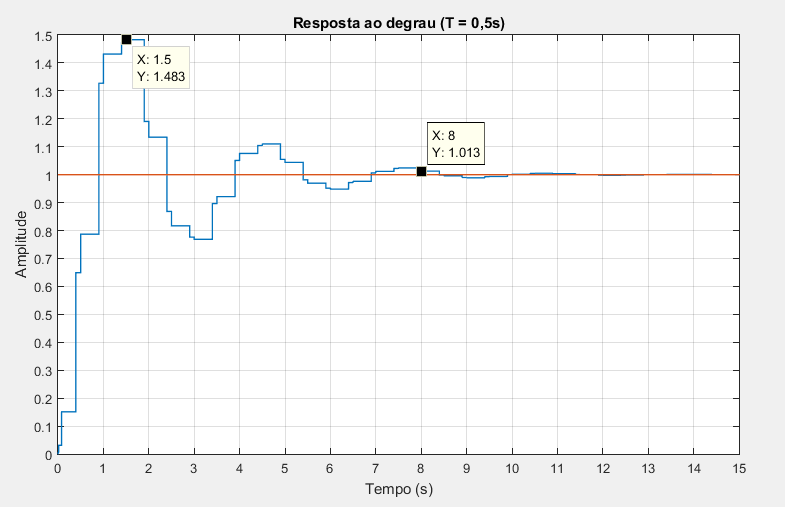
\includegraphics[width=1\linewidth]{images/rDeg05.png}
            \caption{Resposta ao degrau unitário para T = 0,5s.}
            \label{fig:rDeg05}
    \end{figure}

    {Para T = 0,5s, o sobressinal $\approx$  48,3\% e o tempo de acomodação $\approx$ 8 segundos.}

    \vspace{7mm}
    \begin{figure}[H]
       \centering
            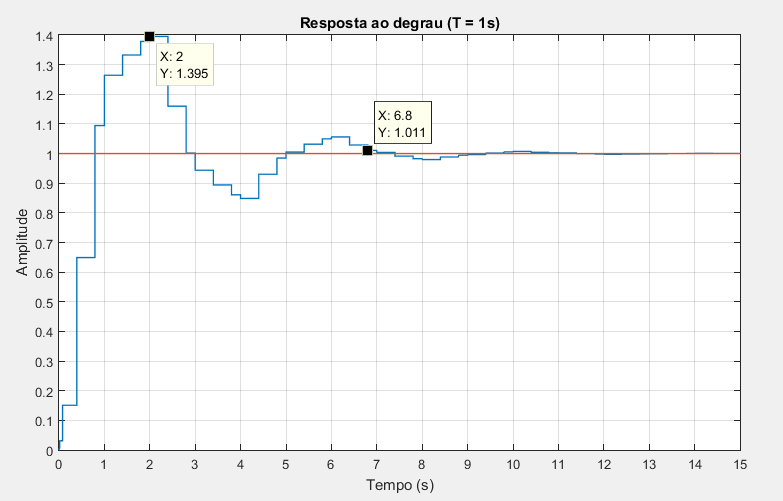
\includegraphics[width=1\linewidth]{images/rDeg1.png}
            \caption{Resposta ao degrau unitário para T = 1s.}
            \label{fig:rDeg1}
    \end{figure}

    {Para T = 1s, o sobressinal $\approx$ 39,5\% e o tempo de acomodação $\approx$ 6,8 segundos.}

    \vspace{7mm}
    \begin{figure}[H]
       \centering
            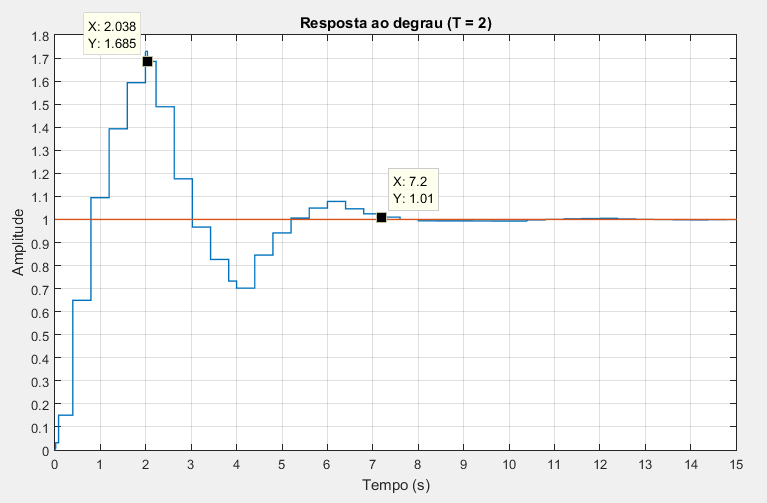
\includegraphics[width=1\linewidth]{images/rDeg2.png}
            \caption{Resposta ao degrau unitário para T = 2s.}
            \label{fig:rDeg2}
    \end{figure}

    {Para T = 2s, o sobressinal $\approx$ 68,5\% e o tempo de acomodação $\approx$ 7,2 segundos.}

    \vspace{14mm}
    {\textbf{e)} As respostas à rampa do sistema para diferentes tempos de amostragem e K = 2 são apresentadas nas figuras a seguir.}

    \begin{figure}[H]
       \centering
            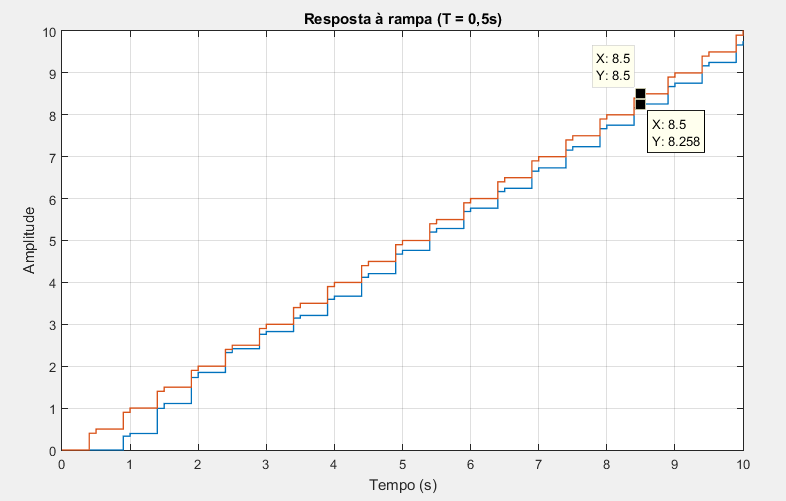
\includegraphics[width=1\linewidth]{images/rRamp05.png}
            \caption{Resposta à rampa para T = 0,5s.}
            \label{fig:rRamp05}
    \end{figure}

    {Para T = 0,5s, o erro em regime permanente Kv para uma entrada rampa $\approx$ 0,242.}

    \vspace{7mm}
    \begin{figure}[H]
       \centering
            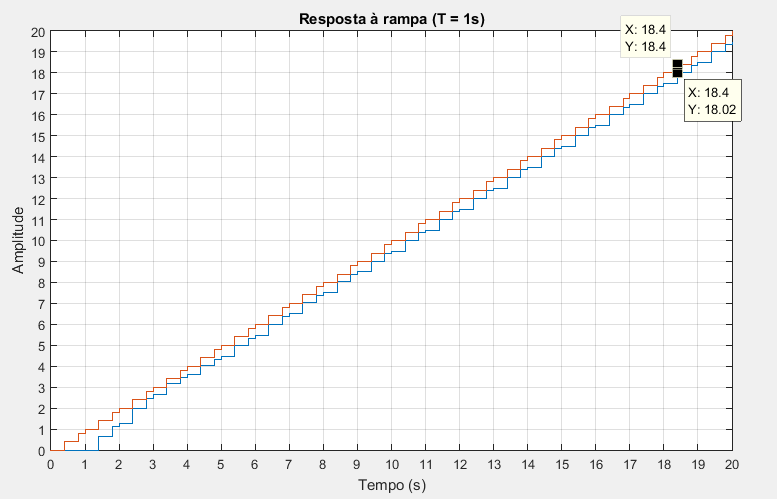
\includegraphics[width=1\linewidth]{images/rRamp1.png}
            \caption{Resposta à rampa para T = 1s.}
            \label{fig:rRamp1}
    \end{figure}

    {Para T = 1s, o erro em regime permanente Kv para uma entrada rampa $\approx$ 0,38.}

    \vspace{7mm}
    \begin{figure}[H]
       \centering
            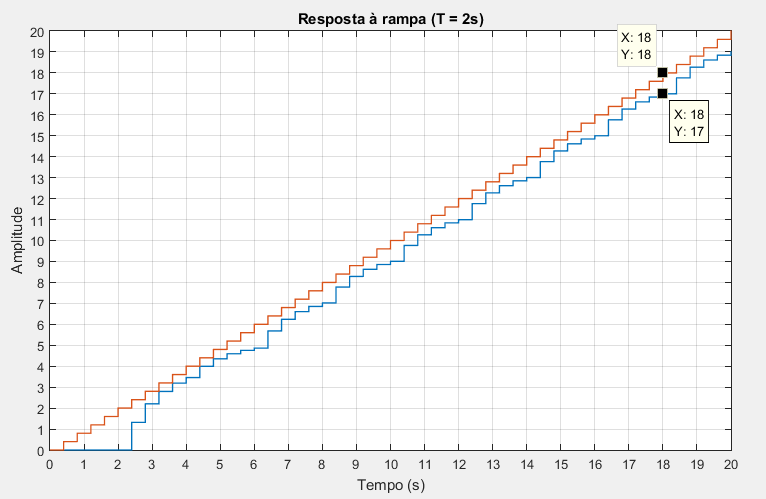
\includegraphics[width=1\linewidth]{images/rRamp2.png}
            \caption{Resposta à rampa para T = 2s.}
            \label{fig:rRamp2}
    \end{figure}

    {Para T = 2s, o erro em regime permanente Kv para uma entrada rampa $\approx$ 1.}

%\newpage
%\section{Questão 2}
%
%    \begin{figure}[H]
%       \centering
%            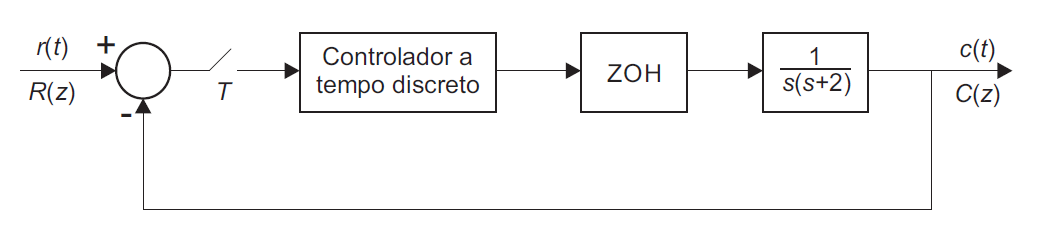
\includegraphics[width=1\linewidth]{Diagrama2.png}
%            \caption{Diagrama do sistema.}
%            \label{fig:diagram2}
%    \end{figure}


\end{document}
